\documentclass{beamer}

% Pacotes utilizados
\usepackage[brazil]{babel}
\usepackage[alf]{abntex2cite}
\usepackage{graphicx,hyperref,url}
\usepackage{uegCCETtheme} % pacote customizado para o curso
\usepackage[T1]{fontenc}
\usepackage[utf8]{inputenc}
\usepackage{ragged2e}
\usepackage{subcaption}
\usepackage{listings}
\usepackage{tikz, tkz-euclide, tkz-fct}
\usetikzlibrary{babel}
\usetkzobj{all}

\renewcommand{\lstlistingname}{Código}
\lstdefinestyle{Python}{
	language={Python},
	basicstyle=\ttfamily\footnotesize,
	identifierstyle=\color{black},
	keywordstyle=\color{blue},
	commentstyle=\color{green},
	stringstyle=\color{red},
	extendedchars=true,
	showspaces=false,
	showstringspaces=false,
	numbers=none,
	breaklines=true,
	backgroundcolor=\color{yellow!20},
	breakautoindent=true,
	captionpos=b,
	xleftmargin=0pt,
	frame=none
}

% Título da apresentação [título curto]{título longo}
\title[Cálculo Variacional e o Método de Rayleigh-Ritz]{Uma Introdução ao Cálculo Variacional e ao Método de Rayleigh-Ritz com Aplicações em Python}
%\subtitle{Apenas um subtítulo}
% Autores da apresentação [nome curto]{nome longo}
\author[Eduardo José de Oliveira]{
	Acadêmico: Eduardo José de Oliveira\\
	Orientador: Prof. Me. Tiago de Lima Bento Pereira
}
% Nome da instituição [nome curto]{nome longo}
\institute[Universidade Estadual de Goiás]{
	UNIVERSIDADE ESTADUAL DE GOIÁS\\
  	Câmpus Anápolis de Ciências Exatas e Tecnológicas Henrique Santillo \\
  	\vfill
  	Curso de Matemática
}
% Data [data curta]{data longa}
\date[2019]{2019}
% Observação: geralmente o título\autor\data curto é usado
%             em locais como o rodapé enquanto que o título
%             longo é usado em lugares como a capa, por exemplo.

% declara ambientes matemáticos
\newtheorem{definicao}{Definição}
\newtheorem{lema}{Lema}

\newcommand{\fonte}[1]{
	\begin{center}
		\footnotesize Fonte: #1
	\end{center}
}

\newcommand{\fonteElaboradoPeloAutor}{
	\fonte{Elaborado pelo autor, 2019.}
}

\newcommand{\fonteElaboradaPeloAutor}{
	\fonte{Elaborada pelo autor, 2019.}
}

\begin{document}

	\begin{frame}[plain]
	  \titlepage
	\end{frame}

	\section{Introdução}
	\begin{frame}
		\frametitle{Introdução}
		
		\justify
		Segundo \citeonline{calcvar} e \citeonline{calcvar_campos}, um dos problemas pertinentes ao Cálculo Variacional é o de minimizar ou maximizar o funcional
		$$
			\int_{x_1}^{x_2} f(x, y, y', y'', \dots, y^{(n)})dx\text{,}
		$$
		isto é, encontrar uma função diferenciável até a ordem $n$, $y=y(x)$, satisfazendo $y(x_1)=y_1$ e $y(x_2)=y_2$, com $x_1$, $x_2$, $y_1$ e $y_2$ dados, tornando a integral um valor mínimo ou máximo.
	\end{frame}
	
	\begin{frame}
		\frametitle{Introdução}
		\justify

		Uma das formas de se encontrar a função $y(x)$ corresponde na determinação da chamada equação de Euler-Lagrange associada ao problema e, então, sua resolução.
		\vspace{10pt}
		\pause
		
		Outra abordagem ao problema consiste na aproximação de $y(x)$ por meio de outras funções, por exemplo, com o Método de Rayleigh-Ritz.
	\end{frame}
	
	\section{Objetivo}
	\begin{frame}
		\frametitle{Objetivos}
	
		\begin{enumerate}
			\justifying
			\item introduzir, de forma clara e concisa, o Cálculo Variacional por meio do estudo das Equações de Euler-Lagrange para funcionais que dependem de uma única variável, da função e das suas derivadas, até a ordem $n$ desejada;
			
			\item explicar o método de Rayleigh-Ritz, de forma simples e introdutória, desenvolvendo exemplos básicos;
			
			\item apresentar formas de se utilizar a computação para os cálculos do método de Rayleigh-Ritz por meio da linguagem de programação Python.
		\end{enumerate}
	\end{frame}

	\section{Contexto Histórico}
	\makesubtitleframe{Contexto Histórico}

	\begin{frame}
		\frametitle{Máximos e Mínimos}
		\justify
	
		Segundo \citeonline{boyer}, tem-se alguns acontecimentos importantes:
		\begin{itemize}
			\justifying
		    \item Pierre de Fermat em 1629.
		    \pause
		    \item Cálculo diferencial em 1665 (Isaac Newton) e 1676 (Gottfried Leibniz).
		\end{itemize}
	\end{frame}

	\begin{frame}
		\frametitle{O Problema da Braquistócrona e o Cálculo Variacional}
		\justify
	
		Segundo \citeonline{hist_courant} e \citeonline{hist_still}, o problema da braquistócrona,
		\begin{itemize}
			\item Foi formulado por Johann Bernoulli em 1696 e pode ser apresentado como:
			\begin{block}{Problema da Braquistócrona}
				Sejam $A$ e $B$ dois pontos dados em um plano vertical. O problema da braquistócrona consiste em encontrar a curva que uma partícula M precisa descrever para sair de A e chegar em B no menor tempo possível, somente sob a ação da força da gravidade \cite[p. 3]{calcvar}.
			\end{block}
		\end{itemize}
	\end{frame}

	\begin{frame}
		\frametitle{O Problema da Braquistócrona e o Cálculo Variacional}
		\justify

		Segundo \citeonline{hist_courant} e \citeonline{hist_still},
		\begin{itemize}
			\item A Solução de Jacob Bernoulli (1697) apresenta o aspecto da curva variável.
			\pause
		
			\item Euler e Lagrange.
		\end{itemize}
	\end{frame}
	
	\begin{frame}
		\frametitle{Método de Rayleigh-Ritz}
		\justify
		
		Segundo \citeonline{LEISSA_2005}, 
		\begin{itemize}
			\justifying
			\item O método leva o nome dos pesquisadores Lord Rayleigh e Walter Ritz.
			\pause
			\item Estudado, primeiro, por Lord Rayleigh com problemas de energias potencial e cinética de sistemas.
			\pause
			\item A Generalização foi feita por Walter Ritz.
			\pause
			\item Não se sabe exatamente quando o método passou a se chamar "Método de Rayleigh-Ritz".
		\end{itemize}
	\end{frame}
	
	\begin{frame}
		\frametitle{Aplicação do Método de Rayleigh-Ritz}
		\justify

		Uma das aplicações mais usuais nos trabalhos acadêmicos é o seu uso para a determinação das chamadas frequências naturais.
		\vspace{10pt}
		\pause
		
		As frequências naturais "indicam a taxa de oscilação livre da estrutura, depois de cessada à força que provocou o seu movimento. Em palavras similares, representa o quanto à estrutura vibra quando não há força aplicada sobre ela."\text{ }\cite[p. 1]{Vasquez2015}.
		\vspace{10pt}
		\pause
		
		\citeonline{deep_ritz} estuda a aplicação do Método junto a Inteligência Aritifical, propondo o método chamado de \textit{Deep Ritz Method} para a resolução de problemas variacionais.
	\end{frame}
	
	\begin{frame}
		\frametitle{Linguagem Python}
		\justify
		
		\begin{itemize}
			\justifying
			\item Criada por Guido van Rossum por volta de 1990.
			\pause
			\item Desenvolvimento \textit{open-source}.
			\pause
			\item Atualmente há cerca de 1000 colaboradores no GitHub.
			\pause
			\item Diversas bibliotecas de rotinas voltadas a computação científica.
%			\item Diversas bibliotecas de rotinas como, por exemplo, o ecossistema SciPy:
%				\begin{itemize}
%					\item NumPy
%					\item SciPy
%					\item MatplotLib
%					\item SymPy\\
%					...
%				\end{itemize}
		\end{itemize}
	\end{frame}

	\section{Cálculo Variacional}
	\makesubtitleframe{Cálculo Variacional}
	
	\begin{frame}
		\frametitle{Cálculo Variacional}
		\justify
		
		Voltando ao problema da introdução, segundo \citeonline{calcvar_campos} e \citeonline{calcvar}, deseja-se encontrar $y=y(x)$, diferenciável até a ordem $n$, com $y(x_1)=y_1$ e $y(x_2)=y_2$ de modo que a integral
		$$
			I = \int_{x_1}^{x_2} f(x, y, y', y'', \dots, y^{(n)})dx
		$$
		seja um valor mínimo ou máximo.
		\vspace{10pt}
		\pause
		
		Variar $y$ por meio de funções admissíveis
		$$
			Y_{\varepsilon}=y(x)+\varepsilon\eta(x)
			\text{.}
		$$
	\end{frame}
	
	\encapsulateBackgroundLessFrames
	{
		\begin{frame}
			\begin{figure}
				\caption{Representação gráfica das funções admissíveis.}
				\begin{center}
					\resizebox{0.5\textwidth}{!}{
						\begin{tikzpicture}
	\tkzInit[xmin=-1, xmax=6, ymin=-1, ymax=6]
	% draw axis without ticks
	\tkzDrawX[noticks]
	\tkzDrawY[noticks]
	
	% define extrems on y(x) curve
	\tkzDefPoint[](2.5, 2.0){A}
	\tkzDefPoint[](4.6, 3.76){B}		
	% define helper points
	\tkzDefPoint[](2.5, 0.0){C}
	\tkzDefPoint[](4.6, 0.0){D}
	\tkzDefPoint[](0.0, 2.0){E}
	\tkzDefPoint[](0.0, 3.76){F}
	% helper points to put labels
	\tkzDefPoint[](3.4, 3.2){G}
	\tkzDefPoint[](2.6, 1.7){H}
	\tkzDefPoint[](3.7, 4.2){I}
	\tkzDefPoint[](3.2, 0.4){J}
	
	% draw extrem points on y(x) curve
	\tkzDrawPoint[fill=black, size=7](A)
	\tkzDrawPoint[fill=black, size=7](B)
		
	% y(x)
	\tkzFct[domain=2.5:4.6,samples=1000, line width=2pt]{-exp(-x+3.2)+4}
	% eta(x)
	\tkzFct[domain=2.5:4.6,samples=1000]{-0.18*x*x+1.29*x-2.09}
	% y(x) + 2*eta(x)
	\tkzFct[domain=2.5:4.6,samples=1000,dashed]{-exp(-x+3.2)+4+2*(-0.18*x*x+1.29*x-2.09)}
	% y(x) - 4*eta(x)
	\tkzFct[domain=2.5:4.6,samples=1000,dashed]{-exp(-x+3.2)+4-4*(-0.18*x*x+1.29*x-2.09)}
		
	% draw dotted segments (x_1, y_1), (x_2, y_2)
	\tkzDrawSegment[dotted](A,C)
	\tkzDrawSegment[dotted](B,D)
	\tkzDrawSegment[dotted](A,E)
	\tkzDrawSegment[dotted](B,F)
		
	% x_1, x_2, y_1, y_2 labels
	\tkzLabelPoint[below](C){$x_1$}
	\tkzLabelPoint[below](D){$x_2$}
	\tkzLabelPoint[left](E){$y_1$}
	\tkzLabelPoint[left](F){$y_2$}
	
	\tkzLabelPoint[right](G){$y(x)$}
	\tkzLabelPoint[right](H){$Y_2(x)=y(x)+\varepsilon _2 \eta(x)$}
	\tkzLabelPoint[right](I){$Y_1(x)=y(x)+\varepsilon _1 \eta(x)$}
	\tkzLabelPoint[right](J){$\eta(x)$}
\end{tikzpicture}
					}\\
					\fonteElaboradaPeloAutor
				\end{center}
				\label{fig:func_approx}
			\end{figure}
		\end{frame}
	}

	\begin{frame}
		\frametitle{Cálculo Variacional}
		\justify
		
		Substituindo $y$ por uma função admissível $Y_{\varepsilon}$, tem-se
		$$
			I(\varepsilon) = \int_{x_1}^{x_2} f(x, Y_{\varepsilon}, Y', Y'', \dots, Y^{(n)})dx
			\text{.}
		$$
		\pause
		
		Fazendo $I'(0)=0$ e realizando as devidas manipulações, obtem-se a equação de Euler-Lagrange
		\begin{block}{Equação de Euler-Lagrange Geral}
			$$
				\sum_{i=0}^n (-1)^i\frac{d^i}{dx^i}\left (
					\frac{\partial f}{\partial y^{(i)}}
				\right )
				= 0
				\text{.}
			$$
		\end{block}
	\end{frame}
	
	\begin{frame}
		\frametitle{Cálculo Variacional}
		\justify

		Um caso mais simples da equação de Euler-Lagrange se dá para o funcional
		$$
			I=\int_{x_1}^{x_2} f(x, y, y')dx
			\text{,}
		$$
		onde a equação é dada por
		
		\begin{block}{Equação de Euler-Lagrange}
			$$
				\frac{\partial f}{\partial y} - \frac{d}{dx} \left ( \frac{\partial f}{\partial y'} \right )=0 \text{.}
			$$
		\end{block}
	\end{frame}
	
	\begin{frame}
		\frametitle{Cálculo Variacional}
		\justify
		
		Um exemplo de uso da equação de Euler-Lagrange
		\pause
		\begin{block}{Curva de Menor Comprimento entre dois Pontos}
			É sabido do cálculo diferencial e integral que o comprimento, $I$, de uma curva $y(x)$ entre dois pontos é determinado por
			$$
				I=\int_{x_1}^{x_2} \sqrt{1+(y'(x))^2} dx
				\text{,}
			$$
			onde $x_1$ e $x_2$ são as abscissas dos dois pontos.
			
			É possível determinar, pela equação de Euler-Lagrange, a curva $y(x)$ com menor comprimento.
		\end{block}
	\end{frame}
	
	\begin{frame}
		\frametitle{Curva de Menor Comprimento entre dois Pontos}
		\justify
		
		Seja
		$$
			\frac{\partial f}{\partial y}
			-
			\frac{d}{dx} \left (
				\frac{\partial f}{\partial y'}
			\right )
			= 0
			\text{,}
		$$
		onde $f(x, y, y')=\sqrt{1+(y'(x))^2}$. \pause Assim,
		$$
			-\frac{d}{dx} \left (
				\frac{y'(x)}{\sqrt{1+(y'(x))^2}}
			\right )
			= 0
		$$
		\pause
		$$
			\frac{y''(x)}{
				\sqrt{1+(y'(x))^2}
			}
			= 0
		$$
		\pause
		$$
			y''(x)=0
			\text{.}
		$$
	\end{frame}
	
	\begin{frame}
		\frametitle{Curva de Menor Comprimento entre dois Pontos}
		\justify
		
		Resolvendo a equação $y''(x)=0$\pause ,
		$$
			\int y''(x)dx = \int 0 dx \Longrightarrow y'(x) = C_1
		$$
		\pause
		$$
			\int y'(x)dx = \int C_1 dx \Longrightarrow y(x) = C_1 x + C_2
		$$
		\pause
		Portanto, $y(x)=C_1 x + C_2$.
	\end{frame}

	%\begin{frame}
	%	\frametitle{Relembrando o problema}
	%	\justify
	%
	%	Deseja-se, no Cálculo Variacional, encontrar uma função diferenciável até segunda ordem $y=y(x)$ satisfazendo $y(x_1)=y_1$ e $y(x_2)=y_2$, com $x_1$, $x_2$, $y_1$ e $y_2$ dados, e $f$ uma função duas vezes diferenciável, minimizando ou maximizando a integral
	%	\begin{equation}
	%		\int_{x_1}^{x_2} f(x,y,y')dx\text{.}
	%		\label{eqn:def_calcvar}
	%	\end{equation}
	%\end{frame}

	%\begin{frame}
	%	\frametitle{Funções Aproximadoras}
	%	\begin{definicao}
	%		\justify
	%		Uma família de funções aproximadoras é definida como
	%		$$Y(x)=y(x)+\varepsilon \eta (x)\text{,}$$
	%		onde a função $\eta (x)$ é uma função diferenciável arbitrária para a qual $\eta (x_1)=\eta (x_2)=0$. O número $\varepsilon$ é o parâmetro da família. Sua derivada pode ser escrita como
	%		$$Y'(x)=y'(x)+\varepsilon \eta '(x)\text{.}$$
	%	\end{definicao}
	%\end{frame}

	
	
	%\begin{frame}
	%	\frametitle{Reescrevendo o Problema}
	%	\justify
	%
	%	Pode-se reescrever a integral \eqref{eqn:def_calcvar} utilizando as funções aproximadoras, dependendo de $\varepsilon$, então
	%	\begin{equation}
	%		\label{eqn:int_funcional_approx}
	%		I(\varepsilon)=\int_{x_1}^{x_2}f(x, Y, Y')dx\text{.}
	%	\end{equation}
	%
	%	Para encontrar a função $y(x)$ que maximiza ou minimiza a integral escrita com as funções aproximadoras \eqref{eqn:int_funcional_approx}, deve-se fazer
	%	$$I'(\varepsilon)=0\text{,}$$
	%	e, considerando que quando $\varepsilon=0$, as integrais \eqref{eqn:def_calcvar} e \eqref{eqn:int_funcional_approx} fornecem os mesmos maximos e mínimos, é necessário que
	%	$$I'(0)=0\text{.}$$
	%\end{frame}

	%\begin{frame}
	%	\justify
	%
	%	Utilizando a Regra de Leibniz, pode-se escrever a derivada de $I(\varepsilon)$ como
	%	$$I'(\varepsilon)=\int_{x_1}^{x_2} \frac{\partial f}{\partial \varepsilon} (x, Y, Y') dx \text{,}$$
	%	\pause
	%	donde, aplicando a regra da cadeia, obtêm-se
	%	$$I'(\varepsilon)=\int_{x_1}^{x_2}\left ( \frac{\partial f}{\partial x}\frac{\partial x}{\partial \varepsilon} + \frac{\partial f}{\partial Y} \frac{\partial Y}{\partial \varepsilon} + \frac{\partial f}{\partial Y'} \frac{\partial Y'}{\partial \varepsilon} \right )dx\text{.}$$
	%	\pause
	%
	%	O primeiro termo do integrando é nulo, pois $x$ independe de $\varepsilon$, então
	%	$$
	%		I'(\varepsilon)=\int_{x_1}^{x_2}\left ( \frac{\partial f}{\partial Y}\frac{\partial Y}{\partial \varepsilon} + \frac{\partial f}{\partial Y'}\frac{\partial Y'}{\partial \varepsilon} \right ) dx \text{.}
	%	$$
	%\end{frame}

	%\begin{frame}
	%	\justify
	%
	%	Derivando a função aproximadora $Y(x)=y(x)+\varepsilon \eta(x)$ em relação a $\varepsilon$, conclui-se que
	%	$$\frac{\partial Y}{\partial \varepsilon}=\eta\text{.}$$
	%	\pause
	%
	%	De modo análogo, ao derivar $Y'(x)=y'(x)+\varepsilon \eta '(x)$ em relação a $\varepsilon$, obtêm-se que
	%	$$\frac{\partial Y'}{\partial \varepsilon}=\eta '\text{.}$$
	%\end{frame}

	%\begin{frame}
	%	\justify
	%
	%	Substituindo $\frac{\partial Y}{\partial \varepsilon}=\eta$ e $\frac{\partial Y'}{\partial \varepsilon}=\eta'$ em $I'(\varepsilon)$,
	%	$$
	%		I'(\varepsilon)=\int_{x_1}^{x_2}\left ( \frac{\partial f}{\partial Y}\frac{\partial Y}{\partial \varepsilon} + \frac{\partial f}{\partial Y'}\frac{\partial Y'}{\partial \varepsilon} \right ) dx
	%	$$
	%	\pause
	%	$$
	%		I'(\varepsilon)=\int_{x_1}^{x_2}\left ( 
	%			\frac{\partial f}{\partial Y} \eta +
	%			\frac{\partial f}{\partial Y'} \eta '
	%		\right )dx \text{.}
	%	$$
	%\end{frame}

	%\begin{frame}
	%	\justify
	%
	%	Calculando $I'(0)$, ou seja, quando $\varepsilon=0$, é possível trocar $Y$ e $Y'$ por $y$ e $y'$, respectivamente, então,
	%	$$
	%		I'(0)=\int_{x_1}^{x_2}\left (
	%			\frac{\partial f}{\partial y} \eta +
	%			\frac{\partial f}{\partial y'} \eta '
	%		\right )dx
	%	$$
	%	\pause
	%	$$
	%		I'(0)=
	%			\int_{x_1}^{x_2} \frac{\partial f}{\partial y}\eta dx
	%			+
	%			\int_{x_1}^{x_2} \frac{\partial f}{\partial y'}\eta' dx \text{.}
	%	$$
	%	\pause
	%
	%	Integrando o segundo membro por partes, tem-se
	%	$$
	%	I'(0)=
	%		\int_{x_1}^{x_2} \frac{\partial f}{\partial y}\eta dx
	%		-
	%		\int_{x_1}^{x_2} \frac{d}{dx} \left ( \frac{\partial f}{\partial y'} \right ) \eta dx
	%	$$
	%\end{frame}
	
	%\begin{frame}
	%	\justify
	%
	%	Organizando $I'(0)$, tem-se
	%	$$
	%		I'(0)=\int_{x_1}^{x_2}\left (
	%			\frac{\partial f}{\partial y} -
	%			\frac{d}{dx}
	%			\left (
	%				\frac{\partial f}{\partial y'}
	%			\right )
	%		\right )\eta dx
	%		\text{.}
	%	$$
	%	\pause
	%	
	%	Devido a condição necessária, $I'(0)=0$, escrevemos
	%	$$
	%		I'(0)=\int_{x_1}^{x_2}\left (
	%			\frac{\partial f}{\partial y} -
	%			\frac{d}{dx}
	%			\left (
	%				\frac{\partial f}{\partial y'}
	%			\right )
	%		\right )\eta dx = 0
	%		\text{.}
	%	$$
	%\end{frame}

	%\begin{frame}
	%	\justify
	%	Para concluirmos a dedução do resultado é necessário o uso do seguinte lema:
	%
	%	\begin{lema}
	%		\justify
	%		Sejam $x_1 < x_2$ fixos e $G(x)$ uma função contínua particular para $x_1 \leqslant x \leqslant x_2$. Se $$\int_{x_1}^{x_2} \eta (x) G(x) dx = 0$$ para cada função diferenciável $\eta (x)$ tal que $\eta (x_1)=\eta (x_2)=0$, concluímos que $G(x)=0$, para todo $x$ de modo que $x_1 \leqslant x \leqslant x_2$.
	%	\end{lema}	
	%
	%\end{frame}

	%\begin{frame}
	%	\frametitle{Equação de Euler-Lagrange}
	%	\justify
	%
	%	Pelo Lema anterior, conlui-se que
	%	$$
	%		\frac{\partial f}{\partial y} - \frac{d}{dx} \left ( \frac{\partial f}{\partial y'} \right )=0 \text{.}
	%	$$
	%	\pause
	%
	%	A equação acima é chamada de \textbf{Equação de Euler-Lagrange}, sendo uma condição necessária para minimizar ou maximizar a integral
	%	$$
	%		\int_{x_1}^{x_2} f(x, y, y')dx \text{.}
	%	$$
	%\end{frame}
	
	%
	% Método de Rayleigh-Ritz
	%
	
	\section{Método de Rayleigh-Ritz}
	\makesubtitleframe{Método de Rayleigh-Ritz}
	
	\begin{frame}
		\frametitle{Método de Rayleigh-Ritz}
		\justify
		
		A determinação da função exata $y(x)$ nem sempre é fácil ou possível. O método de Rayleigh-Ritz, segundo \cite{mefassan} e \cite{MRR_Deflex}, propõe que a função $y(x)$ seja substituida por uma função aproximadora $v(x)$.
		\vspace{10pt}
		\pause
		
		Considere o funcional
		$$
			I = \int_{x_1}^{x_2} f(x, y, y', y'', \dots, y^{(n)})dx\text{,}
		$$
		com as condições de contorno $y(x_1)=y(x_2)=0$.
	\end{frame}
	
	\begin{frame}
		\frametitle{Método de Rayleigh-Ritz}
		\justify
		
		Seja
		$$
			y(x) \approx v(x)=\sum_{i=1}^n a_i \phi_i(x)
			\text{,}
		$$
		onde os $a_i\in\mathbb{R}$ são chamados de parâmetros de deslocamento e as $\phi_i(x)$ são funções de forma e devem ser linearmente independente.
		\vspace{10pt}
		\pause
		
		Substituindo $y$ por $v$ no funcional, tem-se $I=I(a_1, a_2, \dots, a_n)$.
		\vspace{10pt}
		\pause
		
		A condição de máximo ou mínimo para $I$ é, agora, que
		$$
			\frac{\partial I}{\partial a_i} = 0
			\text{,}
		$$
		onde $i=1,2,\dots,n$.
	\end{frame}
	
	% Exemplo
	\encapsulateBackgroundLessFrames{
	\begin{frame}
		\frametitle{Método de Rayleigh-Ritz}
		\justify
		
		\begin{itemize}
			\begin{columns}
				\begin{column}{0.5\textwidth}
					\begin{block}{Exemplo}
						\justify
						\begin{scriptsize}
						Uma viga prismática possui o funcional de energia potencial total associado
						$$
							\Pi = 
							\frac{1}{2} \int_0^l EI \left [
								\frac{d^2v}{dx^2}
							\right ]^2 dx
							-
							\int_0^l qvdx
						$$
						onde $E$ é o módulo de Young do material e I é o momento de inércia da seção transversal da viga em relação ao eixo baricêntrico. Deseja-se encontrar uma função $\overline{v}(x)$ que aproxime a função exata $v(x)$ minimizando ou maximizando o funcional $\Pi$.
						\end{scriptsize}
					\end{block}
				\end{column}
				\begin{column}{0.5\textwidth}
					\begin{figure}[h]
						\caption{Viga prismática.}
						\centering
						\resizebox{\textwidth}{!}{
						\begin{tikzpicture}
							\tkzInit[xmin=-0, xmax=6, ymin=-0.6, ymax=2]
							% draw axis without ticks
							\tkzDrawX[label=$x$, noticks, loosely dashed]
							\tkzDrawY[label=$v(x)$, noticks]
							
							% rectangle
							\tkzDefPoints{
								0/0.6/V_1,
								5/0.6/V_2,
								5/-0.6/V_3,
								0/-0.6/V_4}
							% complete x axis without dashed line
							\tkzDefPoints{
								5/0/A_1,
								6.35/0/A_2}
							% left base triangle
							\tkzDefPoints{
								0/-0.6/T1_1, 
								-0.25/-1.1/T1_2, 
								0.25/-1.1/T1_3}
							% right base triangle
							\tkzDefPoints{
								5/-0.6/T2_1, 
								4.75/-1.1/T2_2,
								5.25/-1.1/T2_3}
							% line on base of right triangle
							\tkzDefPoints{
								4.75/-1.2/T2_B1,
								5.25/-1.2/T2_B2}
							% length marker in bottom
							\tkzDefPoints{
								0/-1.5/L_1,
								0/-2/L_2,
								5/-1.5/L_3,
								5/-2/L_4,
								0/-1.75/LS_1,
								5/-1.75/LS_2}
							
							\tkzDrawSegment[color=black, line width=0.5mm](A_1, A_2)
							
							\tkzDrawPolygon[draw=black](T1_1, T1_2, T1_3)
							\tkzDrawPolygon[draw=black](T2_1, T2_2, T2_3)
							\tkzDrawSegment[color=black](T2_B1, T2_B2)
							\tkzDrawPolygon[draw=black](V_1, V_2, V_3, V_4)
							% q arrows
							\foreach \i in {1,...,25}{
								\tkzDefPoint(0.2*\i,1.3){A_\i}
								\tkzDefPoint(0.2*\i,0.7){B_\i}
								\draw[line width=0.6pt, black,-stealth] (A_\i) -- (B_\i);
							}
							% q text
							\node at (2.5,1.7) {$q$};
							% length marker in bottom
							\tkzDrawSegment[color=black](L_1, L_2)
							\tkzDrawSegment[color=black](L_3, L_4)
							\tkzDrawSegment[color=black](LS_1, LS_2)
							\node at (2.5,-2) {$l$};
						\end{tikzpicture}
						}
						\\
						\fonte{\citeonline[p. 25]{mefassan}.}
					\end{figure}
				\end{column}
			\end{columns}
		\end{itemize}
	\end{frame}
	}
		
	% Resolução do Exemplo
%	\begin{frame}
%		\frametitle{Método de Rayleigh-Ritz}
%		\justify
%		
%		Seja $v_1(x)=a_0 + a_1 x + a_2 x^2$. \pause Das condições de contorno
%		$$
%			v_1(0)=0\Longrightarrow a_0 = 0\text{,}
%		$$
%		\pause
%		$$
%			v_1(l)=0\Longrightarrow a_1 = -a_2l\text{.}
%		$$
%		\pause
%		Logo, $v_1(x)=a_2(x^2-lx)$, \pause $v_1'(x)=a_2(2x-l)$ \pause e $v_1''(x)=2a_2$.
%	\end{frame}
%	
%	\begin{frame}
%		\frametitle{Método de Rayleigh-Ritz}
%		\justify
%		
%		Substituindo $v$ por $v_1$ em $\Pi$,
%		$$
%			\Pi =
%			\frac{1}{2}
%			\int_0^l 4 EI a_2 ^2 dx
%			-
%			\int_0^l q a_2 (x^2-lx) dx
%			\text{.}
%		$$
%		\pause
%		
%		Da condição de estacionariedade, $\dfrac{\partial \Pi}{\partial a_2}=0$,
%		$$
%			a_2 = -\frac{ql^2}{24EI}
%			\text{.}
%		$$
%		\pause
%		E, como $a_1=-a_2l$,
%		$$
%			a_1 = \frac{ql^3}{24EI}
%			\text{.}
%		$$
%	\end{frame}
%	
%	\begin{frame}
%		\frametitle{Método de Rayleigh-Ritz}
%		\justify
%		
%		Assim, 
%		$$
%			v_1(x)=\dfrac{ql^3}{24EI}x - \dfrac{ql^2}{24EI}x^2
%			\text{.}
%		$$
%		\pause
%		
%		Calculando o valor de máxima deflexão,
%		$$
%			v_1\left ( \frac{l}{2} \right )
%			= \frac{ql^4}{96EI}
%			\text{.}
%		$$
%		\pause
%		
%		O valor de máxima deflexão para $v_1(x)$ é menor que o valor exato,
%		$$
%			v\left ( \frac{l}{2} \right )
%			= \frac{5ql^4}{384EI}
%			\text{.}
%		$$
%	\end{frame}
	
%	\begin{frame}
%		\frametitle{Método de Rayleigh-Ritz}
%		\justify
%		
%		Seja $v_2(x)=a_0 + a_1 x + a_2 x^2 + a_3 x^3$. \pause Das condições de contorno
%		$$
%			v_2(0)=0\Longrightarrow a_0 = 0\text{,}
%		$$
%		\pause
%		$$
%			v_2(l)=0\Longrightarrow a_1 = -a_2l - a_3l^2\text{.}
%		$$
%		\pause
%		Logo, 
%		$$v_2(x)=a_2(x^2-lx)+a_3(x^3-l^2x)\text{,}$$
%		\pause 
%		$$v_2'(x)=a_2(2x-l)+a_3(3x^2-l^2)\text{,}$$
%		\pause
%		$$v_2''(x)=2a_2 + 6a_3x\text{.}$$
%	\end{frame}
%	
%	\begin{frame}
%		\frametitle{Método de Rayleigh-Ritz}
%		\justify
%		
%		Substituindo $v$ por $v_2$ em $\Pi$,
%		$$
%			\Pi=
%			\frac{1}{2}
%			\int_0^l
%				\left (
%					EI(2a_2+6a_3x)^2
%				\right ) dx
%			-
%			\int_0^l
%				q
%				\left (
%					a_2(x^2-lx)
%					+
%					a_3(x^3-l^2x)
%				\right ) dx
%			\text{.}
%		$$
%		\pause
%		Da condição de estacionariedade, tem-se o sistema
%		$$
%			\begin{cases}
%				\dfrac{\partial \Pi}{\partial a_2}=0\\[10pt]
%				\dfrac{\partial \Pi}{\partial a_3}=0
%			\end{cases}
%			\text{.}
%		$$
%	\end{frame}
%	
%	\begin{frame}
%		\frametitle{Método de Rayleigh-Ritz}
%		\justify
%		
%		$$
%			\begin{cases}
%				2a_2+3a_3l=\dfrac{-ql^2}{12EI}\\[10pt]
%				2a_2+4a_3l=\dfrac{-ql^2}{12EI}
%			\end{cases}
%			\text{.}
%		$$
%		\pause
%		Resolvendo o sistema,
%		$$
%			a_3=0
%			\text{,}
%		$$
%		\pause
%		$$
%			a_2=-\frac{ql^2}{24EI}
%			\text{.}
%		$$
%	\end{frame}
	
	\begin{frame}
		\frametitle{Método de Rayleigh-Ritz}
		\justify
		
		Considere a função aproximadora $v_3(x)=a_0 + a_1 x + a_2 x^2 + a_3 x^3 + a_4 x^4$. \pause Das condições de contorno essenciais
		$$
			v_3(0)=0\Longrightarrow a_0 = 0\text{,}
		$$
		\pause
		$$
			v_3(l)=0\Longrightarrow a_1 = -a_2l - a_3l^2 - a_4l^3\text{.}
		$$
		\pause
		Logo, 
		$$v_3(x)=a_2(x^2-lx)+a_3(x^3-l^2x) + a_4(x^4-l^3x)\text{,}$$
		\pause 
		$$v_3'(x)=a_2(2x-l)+a_3(3x^2-l^2)+a_4(4x^3-l^3)\text{,}$$
		\pause
		$$v_3''(x)=2a_2 + 6a_3x + 12a_4x^2\text{.}$$
	\end{frame}
	
	\begin{frame}
		\frametitle{Método de Rayleigh-Ritz}
		\justify
		
		Substituindo $v$ por $v_3$ em $\Pi$,
		\begin{multline*}
			\Pi = \frac{1}{2} \int_0^l \left [
				EI(2a_2+6a_3x+12a_4x^2)^2
			\right ] dx
			-
			\\
			-
			\int_0^l q \left [
				a_2(x^2 - lx)
				+
				a_3(x^3 - l^2x)
				+
				a_4(x^4 - l^3x)
			\right ] dx
			\text{.}
		\end{multline*}
	\end{frame}
	
	\begin{frame}
		\frametitle{Método de Rayleigh-Ritz}
		\justify
		Da condição de estacionariedade, tem-se o sistema
		$$
			\begin{cases}
				\dfrac{\partial \Pi}{\partial a_2}=0\\[10pt]
				\dfrac{\partial \Pi}{\partial a_3}=0\\[10pt]
				\dfrac{\partial \Pi}{\partial a_4}=0
			\end{cases}
			\text{.}
		$$
	\end{frame}
	
	\begin{frame}
		\frametitle{Método de Rayleigh-Ritz}
		\justify
		
		$$
			\begin{cases}
				2a_2 + 3a_3l + 4a_4l^2 = -\dfrac{ql^2}{12EI}\\[10pt]
				a_2 + 2a_3 l + 3a_4 l^2 = - \dfrac{ql^2}{24EI}\\[10pt]
				8a_2 + 18a_3 l + \dfrac{144}{5} a_4 l^2 =-\dfrac{3ql^2}{10EI}
			\end{cases}
		$$
		\pause
		Resolvendo o sistema, tem-se
		$$
			a_2 = 0
			\text{,}
		$$
		\pause
		$$
			a_3 = -\frac{ql}{12EI}
			\text{,}
		$$
	\end{frame}
	
	\begin{frame}
		\frametitle{Método de Rayleigh-Ritz}
		\justify
	
		$$
			a_4 = \frac{q}{24EI}
			\text{.}
		$$
		\pause
		Como $a_1=-a_2l - a_3l^2-a_4l^3$,
		$$
			a_1 = \frac{ql^3}{24EI}
			\text{.}
		$$
		\pause
		A função $v_3$ é
		$$
			v_3(x)=
			\frac{ql^3}{24EI} x
			-
			\frac{ql}{12EI} x^3
			+
			\frac{q}{24EI} x^4
			\text{.}
		$$
	\end{frame}
	
	\begin{frame}
		\frametitle{Método de Rayleigh-Ritz}
		\justify
		
		O resultado analítico do exemplo é
		$$
			v(x)=\frac{ql^3}{24EI}x - \frac{ql}{12EI}x^3 + \frac{q}{24EI}x^4
			\text{,}
		$$
		\pause
		sendo a máxima deflexão da viga
		$$
			v\left (\frac{l}{2}\right )
			=
			v_3\left (\frac{l}{2}\right )
			= \frac{5ql^4}{384EI}
			\text{.}
		$$
		\pause
		
		Comparando as funções $v_3(x)$ e $v(x)$ percebe-se que o resultado encontrado pelo Método de Rayleigh-Ritz e o resultado analítico são iguais.
	\end{frame}
	
	\begin{frame}
		\frametitle{Funções Triangulares}
		\justify
		
		\citeonline{MRR_Deflex} apresenta o seguinte problema
		\begin{block}{Exemplo}
			\justify
			
			Considere o funcional
			$$
				I = \int_{0}^{1} \left [ 
					p(x) \left ( 
						\frac{dy}{dx}
					\right )^2
					+ q(x)(y(x))^2 
					- 2f(x)y(x) 
				\right ] dx
				\text{,}
			$$
			associado ao Problema de Valor de Contorno que modela a deflexão de uma viga apoiada sobre seus extremos. Deseja-se encontrar $y=y(x)$ que maximiza ou minimiza o funcional $I$.
		\end{block}
	\end{frame}
	
	\encapsulateBackgroundLessFrames{
	\begin{frame}
		\frametitle{Funções Triangulares}
		\justify
		
		\begin{itemize}
			\begin{columns}
				\begin{column}{0.55\textwidth}
			   		Considere a função de forma
			   		$$
			   			\phi_i (x) = 
							\begin{cases}
								0 							& \mbox{se } 0 \leqslant x \leqslant x_{i - 1}\\[5pt]
								\dfrac{x-x_{i-1}}{h_{i-1}} 	& \mbox{se } x_{i-1} < x \leqslant x_i\\[10pt]
								\dfrac{x_{i+1}-x}{h_i}		& \mbox{se } x_i < x \leqslant x_{i+1}\\[5pt]
								0							& \mbox{se } x_{i+1}<x\leqslant 1
							\end{cases}
			   		$$
			   		onde $h_i = x_{i+1}-x_{i}$ e $h_{i-1}=x_i-x_{i-1}$.
				\end{column}\pause
				\begin{column}{0.45\textwidth}
					\begin{figure}
						\caption{Função Triangular $\phi_i(x)$}
						\resizebox{0.9\textwidth}{!}{
							\begin{tikzpicture}
								\tkzInit[xmin=-0, xmax=10, ymin=0, ymax=6.4]
								% desenhar os eixos sem marcação
								\tkzDrawX[label={$x$}, noticks]
								\tkzDrawY[label={$y(x)=\phi_i(x)$}, noticks]
								
								% pontos da caixa
								\tkzDefPoints{
									0/0/C_1,
									10/0/C_2,
									10/6/C_3,
									0/6/C_4}
								% desenho da caixa
								%\tkzDrawSegment[color=black, line width=0.5mm, loosely dashed](C_1, C_2)
								\tkzDrawSegment[color=black, line width=0.5mm, loosely dashed](C_2, C_3)
								\tkzDrawSegment[color=black, line width=0.5mm, loosely dashed](C_3, C_4)
								%\tkzDrawSegment[color=black, line width=0.5mm, loosely dashed](C_4, C_1)
								
								% pontos da função
								\tkzDefPoints{
									0/0/F_0,
									4/0/F_1,
									6/6/F_2,
									7/0/F_3,
									10/0/F_4}
								% desenho da função
								\tkzDrawSegment[color=black, line width=0.7mm](F_0, F_1)	
								\tkzDrawSegment[color=black, line width=0.7mm](F_1, F_2)
								\tkzDrawSegment[color=black, line width=0.7mm](F_2, F_3)
								\tkzDrawSegment[color=black, line width=0.7mm](F_3, F_4)
								
								% textos das marcas: x_{i-1}, x_i, x_{i+1}
								\node at (4, -0.5) {$x_{i-1}$};
								\node at (6, -0.5) {$x_{i}$};
								\node at (7, -0.5) {$x_{i+1}$};
								
								% linha (pontilhada) em x_i
								\tkzDefPoints{
									6/0/PT_1,
									6/6/PT_2}
								\tkzDrawSegment[color=black, line width=0.5mm, dashed](PT_1, PT_2)
								
								% nome da função $\phi_i(x)$
								\node at (4, 3) {$\phi_i(x)$};
								
								% marcador dos intervalos $h_{i-1}$, $h_i$
								\node at (5, -1.2) {$h_{i-1}$};
								\tkzDefPoints{
									4/-0.8/M_1,
									4/-0.7/M_11,
									4/-0.9/M_12,
									6/-0.8/M_2,
									6/-0.7/M_21,
									6/-0.9/M_22,
									7/-0.8/M_3,
									7/-0.7/M_31,
									7/-0.9/M_32}
								\tkzDrawSegment[color=black, line width=0.5mm](M_1, M_2)
								\tkzDrawSegment[color=black, line width=0.5mm](M_11, M_12)
								\tkzDrawSegment[color=black, line width=0.5mm](M_21, M_22)
								\tkzDrawSegment[color=black, line width=0.5mm](M_2, M_3)
								\tkzDrawSegment[color=black, line width=0.5mm](M_31, M_32)
								\node at (6.5, -1.2) {$h_i$};
								\node at (-0.2, 6) {$1$};
							\end{tikzpicture}
						}
						\fonteElaboradaPeloAutor
					\end{figure}
				\end{column}
			\end{columns}
		\end{itemize}
	\end{frame}
	}
	
	\begin{frame}
		\frametitle{Funções Triangulares}
		\justify
		
		Substituindo a função aproximadora
		$$
			v(x)=\sum_{i=1}^n a_i \phi_i (x)
		$$
		no funcional $I$, tem-se
		\begin{multline*}
			I = \int_{0}^{1} \left [
				p(x) \left (
					\sum_{i=1}^{n} a_i \phi_i '(x)
				\right )^2
				+ q(x) \left (
					\sum_{i=1}^{n} a_i \phi_i (x)
				\right )^2
			\right ] dx -
			\\
			- \int_{0}^{1} \left [
				- 2f(x) \left (
					\sum_{i=1}^{n} a_i \phi_i (x)
				\right )
			\right ] dx
			\text{.}
		\end{multline*}
	\end{frame}
	
	\begin{frame}
		\frametitle{Funções Triangulares}
		\justify
		
		Aplicando a condição de estacionariedade
		$$
			\frac{\partial I}{\partial a_j} = 0
			\text{,}
		$$
		onde $j=1,2,\dots,n$ e fazendo as devidas manipulações chega-se no sistema
		\pause
		$$
			M\cdot A = B
			\text{,}
		$$
		\pause
		com $M=[m_{j,i}]$, $A=[a_j]$, $B=[b_j]$ e
		$$
			m_{j,i}=\int_{0}^{1} \left [
				2p(x)\phi_i'(x)\phi_j'(x)
				+
				2q(x)\phi_i(x)\phi_j(x)
			\right ]dx
			\text{,}
		$$
		$$
			b_j=\int_{0}^{1} 2f(x)\phi_j(x)dx
			\text{.}
		$$
	\end{frame}
	
	\section{Método de Rayleigh-Ritz e a Linguagem Python}
	\makesubtitleframe{Utilizando o Método de Rayleigh-Ritz na Linguagem Python}

	\begin{frame}
		\frametitle{Método de Rayleigh-Ritz e a Linguagem Python}
		\justify
		
		Considere o funcional
		$$
			\Pi = 
			\frac{1}{2} \int_0^l EI \left [
				\frac{d^2v}{dx^2}
			\right ]^2 dx
			-
			\int_0^l qvdx
			\text{,}
		$$
		do Exemplo sobre o Método de Rayleigh-Ritz.
		\vspace{10pt}
		\pause
		
		Seja a função aproximadora $v_3(x)$,
		$$
			v_3(x)=a_0 + a_1 x + a_2 x^2 + a_3 x^3 + a_4 x^4
			\text{.}
		$$
	\end{frame}
	
	\begin{frame}[containsverbatim]
		\begin{lstlisting}[style=Python,numbers=left, caption={Definição da Função Aproximadora e Integrando}, captionpos=t]
from sympy import symbols, integrate, diff, Matrix
from sympy.solvers import solve

l, E, I, x, q = symbols('l E I x q')
a2, a3, a4 = symbols("a2 a3 a4")

v = a2 * (x**2 - l*x) 
v = v + a3 * (x**3 - l**2 * x)
v = v + a4 * (x**4 - l**3 * x)

dv = diff(v, x)
dv2 = diff(dv, x)

f = (E*I*((dv2)**2)) / 2 - q * v
		\end{lstlisting}
		\fonteElaboradoPeloAutor
	\end{frame}
	
	\begin{frame}
		\frametitle{Método de Rayleigh-Ritz e a Linguagem Python}
		\justify
		
		Para encontrar os parâmetros $a_2$, $a_3$ e $a_4$, resolve-se o sistema
		$$
			\begin{cases}
				\dfrac{\partial \Pi}{\partial a_2}=0\\[10pt]
				\dfrac{\partial \Pi}{\partial a_3}=0\\[10pt]
				\dfrac{\partial \Pi}{\partial a_4}=0
			\end{cases}
			\text{.}
		$$
	\end{frame}
	
	\begin{frame}[containsverbatim]
		\begin{lstlisting}[style=Python, numbers=left, firstnumber=15, caption={Resolvendo o Sistema de Equações}, captionpos=t]

df_a2 = diff(f, a2)
df_a3 = diff(f, a3)
df_a4 = diff(f, a4)

eq1 = integrate(df_a2, (x, 0, l))
eq2 = integrate(df_a3, (x, 0, l))
eq3 = integrate(df_a4, (x, 0, l))

sol = solve([eq1, eq2, eq3], [a2, a3, a4])
print(sol)
		\end{lstlisting}
		\fonteElaboradoPeloAutor
	\end{frame}
	
	\encapsulateBackgroundLessFrames{
	\begin{frame}
		\begin{figure}
			\caption{Resultado encontrado para $a_2$, $a_3$ e $a_4$}
			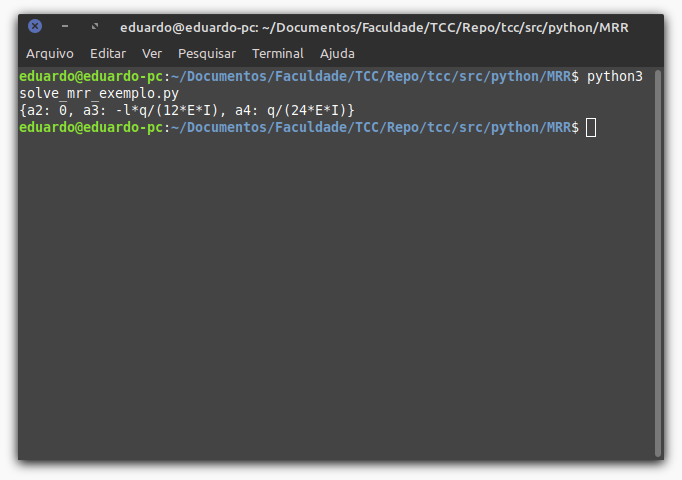
\includegraphics[scale=1.8]{../figuras/code/code_solve_mrr_exemplo_livro.png}
			\fonteElaboradaPeloAutor
			%\\{\footnotesize Fonte: Elaborada pelo autor, 2019.}
		\end{figure}
	\end{frame}
	}
	
	\begin{frame}[containsverbatim]
		\begin{lstlisting}[style=Python, numbers=left, firstnumber=26, caption={Determinando o coeficiente $a_1$}, captionpos=t]
a1 = -a2*l - a3*l**2 - a4 * l**3
a1 = a1.subs(a2, sol[a2])
a1 = a1.subs(a3, sol[a3])
a1 = a1.subs(a4, sol[a4])
print("a1: ", a1)
		\end{lstlisting}
		\fonteElaboradoPeloAutor
		\vspace{-10pt}
		\begin{lstlisting}[style=Python, numbers=left, firstnumber=31, caption={Determinando a função $v$ e a Máxima Deflexão}, captionpos=t]
v = a1*x + sol[a2]*x**2 + sol[a3]*x**3 + sol[a4]*x**4
print("v(x) = ", v)
maxdef = v.subs(x, l/2)
print("Maxima deflexao: ", maxdef)
		\end{lstlisting}
		\fonteElaboradoPeloAutor
	\end{frame}
	
	\encapsulateBackgroundLessFrames{
	\begin{frame}
		\begin{figure}
			\caption{Execução completa dos Códigos 1, 2, 3 e 4}
			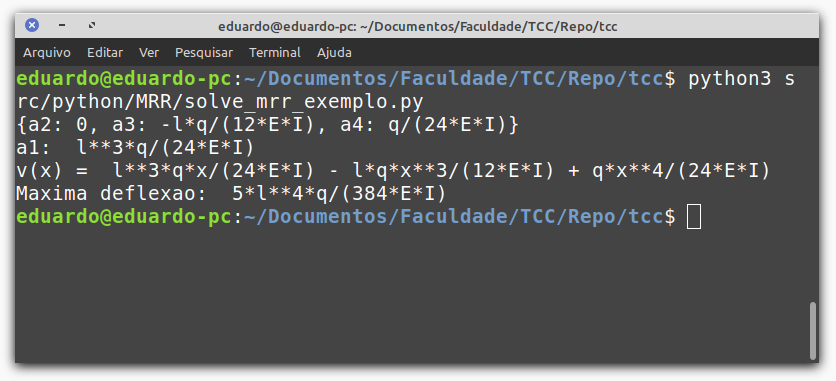
\includegraphics[scale=0.38]{../figuras/code/code_solve_mrr_exemplo_livro_presentation_zoom.png}
			\vspace{-10pt}
			\fonteElaboradaPeloAutor
		\end{figure}
	\end{frame}
	}
	
	\begin{frame}
		\frametitle{Funções Triangulares na Linguagem Python}
		\justify
	
		O problema da viga apoiada dado na Seção sobre o uso de Funções Triangulares no Método de Rayleigh-Ritz, resultou no sistema $$M\cdot A=B$$ com $M=[m_{j,i}]$, $A=[a_j]$ e $B=[b_j]$, onde
		$$
			m_{j,i}=\int_{0}^{1} \left [
				2p(x)\phi_i'(x)\phi_j'(x)
				+
				2q(x)\phi_i(x)\phi_j(x)
			\right ]dx
			\text{,}
		$$
		$$
			b_j=\int_{0}^{1} 2f(x)\phi_j(x)dx
			\text{.}
		$$
		\pause
		Esse sistema pode ser resolvido numericamente utilizando a linguagem Python.
	\end{frame}
	
	\begin{frame}
		\frametitle{Funções Triangulares na Linguagem Python}
		\justify
		
		O funcional do problema é
		$$
			I = \int_{0}^{1} \left [ 
					p(x) \left ( 
						\frac{dy}{dx}
					\right )^2
					+ q(x)(y(x))^2 
					- 2f(x)y(x) 
				\right ] dx
				\text{,}
		$$
		\pause
		e para comparação, serão utilizadas as funções
		\begin{itemize}
			\item $p(x)=e^x$;
			\item $q(x)=e^x$;
			\item $f(x)=x+(2-x)e^x$.
		\end{itemize}
		\pause
		
		Para essas funções, a função exata é conhecida
		$$
			y(x)=(x-1)(e^{-x}-1)
			\text{.}
		$$
	\end{frame}
	
	%\begin{frame}
	%	\frametitle{Funções Triangulares na Linguagem Python}
	%	\justify
	%	
	%	sdas
	%\end{frame}
	
	\begin{frame}[containsverbatim]
		\vspace{-8pt}
		\begin{lstlisting}[style=Python, numbers=none, caption={Trechos do código sobre funções triangulares}, captionpos=t]
#[...]
n = 5
space = 1/(n + 1)
intervals = numpy.arange(0, 1.0001, space)

def fi(i, x):
    if x <= intervals[i - 1]:
        return 0
    elif x <= intervals[i]:
        h = (intervals[i] - intervals[i - 1])
        return ((x - intervals[i - 1]) / h)
    elif x <= intervals[i + 1]:
        h = (intervals[i + 1] - intervals[i])
        return ((intervals[i + 1] - x) / h)
    else:
        return 0
		\end{lstlisting}
		\fonteElaboradoPeloAutor
	\end{frame}
	
	\begin{frame}[containsverbatim]
		\begin{lstlisting}[style=Python, numbers=none, caption={Trechos do código sobre funções triangulares}, captionpos=t]
#[...]
M = zeros(n, n+1)
for i in range(0, n):
    M[i, n] = b(i)
    M[i, i] = m(i, i)
    if (i - 1) >= 0:
        M[i, i - 1] = m(i, i - 1)
    if (i + 1) < n:
        M[i, i + 1] = m(i, i + 1)
coeficients = symbols('a_0:{}'.format(n))
solution, = linsolve(M, coeficients)
		\end{lstlisting}
		\fonteElaboradoPeloAutor
	\end{frame}
	
	\encapsulateBackgroundLessFrames{
		\begin{frame}
			\begin{figure}
				\caption{Resolução do Exemplo com 5 segmentos}
				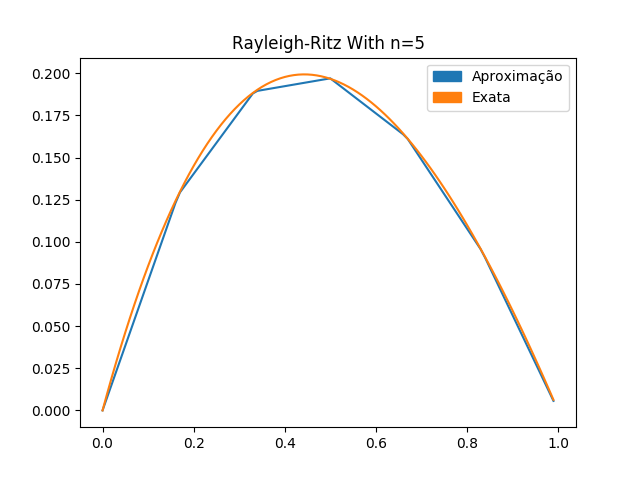
\includegraphics[scale=0.45]{../figuras/code/code_plot_mrr_triangulate.png}
				\fonteElaboradaPeloAutor
			\end{figure}
		\end{frame}
		
		\begin{frame}
			\begin{figure}
				\caption{Resolução do Exemplo com 10 segmentos}
				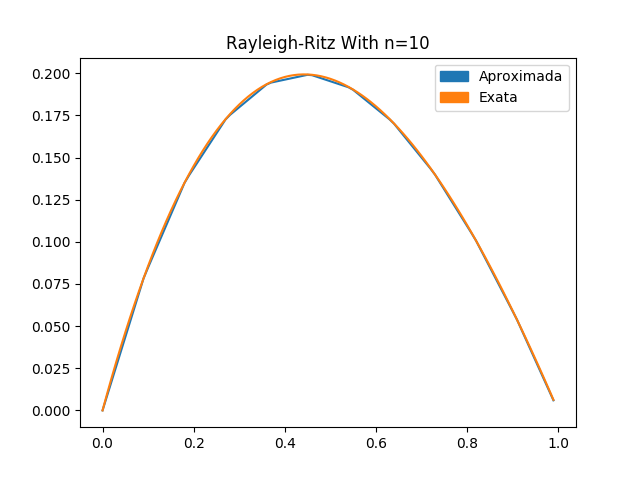
\includegraphics[scale=0.45]{../figuras/code/code_plot_mrr_triangulate_n10.png}
				\fonteElaboradaPeloAutor
			\end{figure}
		\end{frame}
	}
		
	%
	% Exibe as referências citadas nos slides
	% Observação: O parâmetro [allowframebreaks]
	%             na frente do ambiente frame
	%             permite que o slide seja quebrado
	%             passando-se a um próximo quando
	%             o conteúdo passar do seu tamanho.
	%
	\section{Referências}
	\makesubtitleframe{Referências}
	\begin{frame}[allowframebreaks]
		\frametitle{Referências}
		\bibliography{../references}
	\end{frame}

	\makesubtitleframe{OBRIGADO!}
\end{document}